\documentclass[tikz,border=50mm]{standalone}
% !TeX program = luatex

%===This is the preambule I call in every file===

\usepackage{tikz}
\usepackage{xcolor}
\usepackage{pgfplots}
\usepackage{circuitikz}
\usepackage{tikz-3dplot}
\pgfplotsset{compat=newest}
\usetikzlibrary{arrows.meta, shapes.geometric, positioning, perspective, patterns.meta, decorations.pathreplacing, decorations.pathmorphing, decorations.markings, patterns, arrows.meta, shapes, shapes.geometric, decorations.text, angles, quotes,calc, 3d, math, circuits.ee.IEC,hobby, knots, intersections, through}


%=== The Euler Med Logo ===
%=== i.e. My signature ===

\usepackage{amsmath, amsfonts}
\makeatletter
\newcommand*\eulermed{{
\scalebox{3.3}{$\mathbb{E}$}\kern-1pt \scalebox{1.5}{u$\ell\varepsilon\rho$}\kern-55pt
\raisebox{19pt}{\scalebox{1.5}{$\mathcal{M}\varepsilon\delta$}}}
\@}
\makeatother

\begin{document}
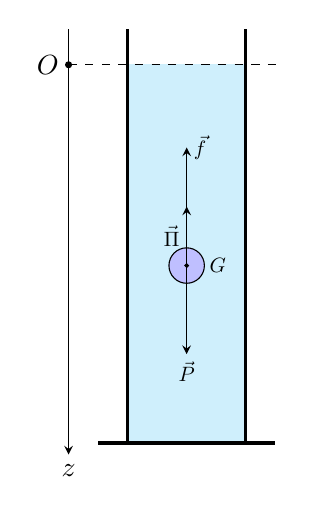
\begin{tikzpicture}[>=stealth, scale=1.5]
%the fluid 
\filldraw[white!75!cyan, opacity=0.75] (-0.5,-3.5)rectangle(0.5,-0.3);
%the sink
\draw[very thick] (-0.5,0)--(-0.5,-3.5) (0.5,0)--(0.5,-3.5);
\draw[ultra thick] (-0.75,-3.5)--(0.75,-3.5);
%the axis
\draw[->] (-1,0)--(-1,-3.6) node[below] {$z$};
\filldraw[black] (-1,-0.3)circle(0.025) node[left] {$O$};
\draw[dashed] (-1,-0.3)--(0.8,-0.3);
%the ball and representation of the forces 
\draw[fill=white!75!blue] (0,-2)circle(0.15) node[right=0.2, scale=0.75] {$G$};
\filldraw[black] (0,-2)circle(0.015);
\draw[->] (0,-2)--(0,-2.75) node[below, scale=0.75] {$\vec{P}$};
\draw[->] (0,-2)--(0,-1.5) node[left,midway,scale=0.75] {$\vec{\Pi}$};
\draw[->] (0,-2)--(0,-1) node[right, scale=0.75] {$\vec{f}$};
\end{tikzpicture}
\end{document}
